\section{Introduction}
\begin{frame}[fragile, allowframebreaks]{Introduction}
\begin{block}{Acknowledgement}
A special thanks to {\bf CeSeNA Security} group and \emph{Marco Ramilli} our ``old'' mentor...
\end{block}
\end{frame}

\subsection{Smash the stack}
\begin{frame}[fragile, allowframebreaks]{Smash the stack}
\begin{block}{\emph{Smash The Stack} [C programming] n.}
On many C implementations it is possible to corrupt the execution stack by writing past the end of an array declared auto in a routine. \\Code that does this is said to smash the stack, and can cause return from the routine to jump to a random address. \\This can produce some of the most insidious data-dependent bugs known to mankind.
\end{block}
\end{frame}
%%%%%%%%%%%%%%%%%%%%%%%%%%%%%%%%%%%%%%%%%%%%%%%%%%%%%%%%%%%%%%%%%%%%%%%%
\subsection{A brief time line}
\begin{frame}[fragile, allowframebreaks]{A brief time line}
\begin{block}{The fist document Overflow Attack (Air Force) - 31/10/1972}
\emph{``By supplying addresses outside the space allocated to the users
programs, it is often possible to get the monitor to obtain unauthorized
data for that user, or at the very least, generate a set of conditions in
the monitor that causes a system crash.''}
\end{block}

\framebreak

\begin{block}{The morris Worm - 2/11/1988}
Robert Tappan Morris (Jr.) wrote and released this while still a student at Cornell University. Aside from being the first computer worm to be distributed via the Internet, the worm was the public’s introduction to \emph{``Buffer Overflow Attacks''}, as one of the worms attack vectors was a classic stack smash against the \emph{fingerd} daemon.\\
In his analysis of the worm, Eugene Spafford writes the following:\\
``\emph{The bug exploited to break fingerd involved {\bf overrunning the buffer} the daemon used for input. \ldots \\
The idea of using buffer overflow to inject code into a program and cause it to jump to that code occurred to me while reading fingerd.c}''
\end{block}

\framebreak

\begin{block}{How to Write Buffer Overflow 20/10/1995}
\emph{by Peiter Zatko (mudge)}\\
``\ldots \\
    \emph{The '{\bf Segmentation fault (core dumped)}' is what we wanted to see. This
    tells us there is definitely an attempt to access some memory address
    that we shouldn't. If you do much in 'C' with pointers on a unix
    machine you have probably seen this (or Bus error) when pointing or
    dereferencing incorrectly.}\\
\ldots ''
\end{block}

\begin{block}{Smashing The Stack For Fun And Profit 8/11/1996}
\emph{by Elias Levy (Aleph1)}\\
One of the best article about BoF.
\end{block}

\end{frame}
%%%%%%%%%%%%%%%%%%%%%%%%%%%%%%%%%%%%%%%%%%%%%%%%%%%%%%%%%%%%%%%%%%%%%%%%
\subsection{Process Memory}
\begin{frame}[fragile, allowframebreaks]{Process Memory}

\begin{block}{Buffers, Memory and Process}
To understand what stack buffers are we must first understand how a
program and process are organized.
\end{block}

\begin{itemize}
\item Program layout is divided in sections like:
	\begin{list}{}{}
		\item .text, where program instruction are stored
		\item .data, where program data will be stored
		\item .bss, where static vars are allocated
		\item .stack, where {\bf stack frames} live
	\end{list}
\item These sections are typically mapped in memory segments, so they have associated RWX permissions.
\end{itemize}

\framebreak

\begin{block}{.text}
The text region is fixed by the program and includes code (instructions) and read-only data.  This region corresponds to the text section of the executable file.  This region is normally marked read-only and any attempt to write to it will result in a \emph{segmentation violation}.
\end{block}
\begin{block}{.data .bss}
The data region contains initialized and uninitialized data. Static variables are stored in this region. The data region corresponds to the data-bss sections of the executable file.  Its size can be changed with the \emph{brk(2)} system call.  If the expansion of the bss-data or the user stack exhausts available memory, the process is blocked and is rescheduled to run again with a larger memory space.\\ 
New memory is added between the data and stack segments.
\end{block}

\framebreak

\begin{verbatim}
  /------------------\ higher
  |                  | memory
  |      Stack       | addresses
  |------------------|
  |  (Uninitialized) |
  |        Data      |
  |   (Initialized)  |
  |------------------|
  |       Text       | lower
  |                  | memory
  \------------------/ addresses
\end{verbatim}
\end{frame}
%%%%%%%%%%%%%%%%%%%%%%%%%%%%%%%%%%%%%%%%%%%%%%%%%%%%%%%%%%%%%%%%%%%%%%%%
\subsection{Stack Frame}
\begin{frame}[fragile, allowframebreaks]{Stack Frame}

\begin{itemize}
\item The stack consists of logical stack frames that are pushed when calling a
function and popped when returning. A stack frame contains the parameters to a
function, its local variables, and the data necessary to recover the previous
stack frame, including the value of the instruction pointer at the time of the
function call.
\item Depending on the implementation the stack will either grow down (towards
lower memory addresses), or up. The stack pointer is also implementation
dependent. It may point to the last address on the stack, or to the next free
available address after the stack. 
\item In addition to the stack pointer, which points to the top of the stack, it
is often convenient to have a frame pointer which points to a fixed location
within a frame. Some texts also refer to it as a local base pointer.
\end{itemize}

\framebreak

\begin{block}{Stack}
In x86 architecture stack grows in opposite direction w.r.t. memory addresses. 
Also two registers are dedicated for stack management.
\begin{description}
\item[EBP/RBP], points to the {\bf base} of the stack-frame (\emph{higher address})
\item[EIP/RIP], points to the {\bf top} of the stack-frame (\emph{lower address})
\end{description}
\end{block}

\framebreak

\begin{block}{Stack Frame}
Logical stack frames that are pushed when calling a function and popped when returning.\\
A stack frame contains:
\begin{itemize}
\item Parameters passed to the called function (depends on calling convention, not true for linux64)
\item {\bf Data necessary to recover the previous stack frame, including value of the instruction pointer at the time of the function call}.
\item Local variables
\end{itemize}
\end{block}

\framebreak

	\begin{figure}
        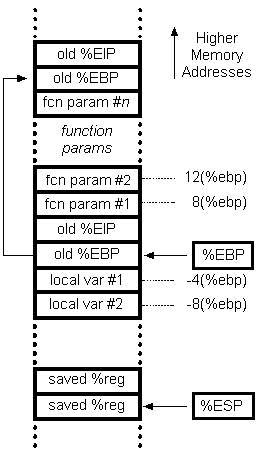
\includegraphics[width=0.4\textwidth]{imgs/stackframe.png}
        \label{fig:stackframe}
        \caption{Stack frame (ia32 - AT\&T notation)}
    \end{figure}	

\framebreak

\begin{block}{Call Prologue and Epilogue}
\begin{columns}[c] 
    \column{.5\textwidth} 
    \acode
    \tiny
\begin{lstlisting}
;params passing*
call fun ;it push EIP/RIP
push EBP
mov EBP,ESP
sub ESP,<param-space>
\end{lstlisting}
    \column{.5\textwidth}
     \acode
     \tiny
\begin{lstlisting}
mov ESP,EBP
pop EBP ;restore old EBP/RBP
ret ;pop EIP/RIP

\end{lstlisting}
\end{columns}
\end{block}


\end{frame}
